%----------------------------------------------------------------------------------------
%	Capítulo 4
%----------------------------------------------------------------------------------------

\pagestyle{myportland}
\pagenumbering{arabic}
\doublespacing
\chapter[----- Antecedentes]{Antecedentes}
\thispagestyle{myportland}

%% NUEVA SECCIÓN X.X
\section{Descripción del sistema conceptual}
\label{sec:descripcion del sistema conceptual}

El presente trabajo es la continuación del trabajo "{Dise{\~{n}}o conceptual de clasificadora y contadora de truchas arco{\'{i}}ris (Oncorhynchus mykiss) de 10 a 20 cent{\'{i}}metros para la crianza de truchas en la Laguna de Paucarcocha}"  \footnote{\cite{DiazVergara2020}}. En la Figura \ref{fig:concepto optimo dibujo y virtual} se muestra el bosquejo del concepto de solución óptimo como su virtualización.

\begin{myfigure}[H]
	\centering
	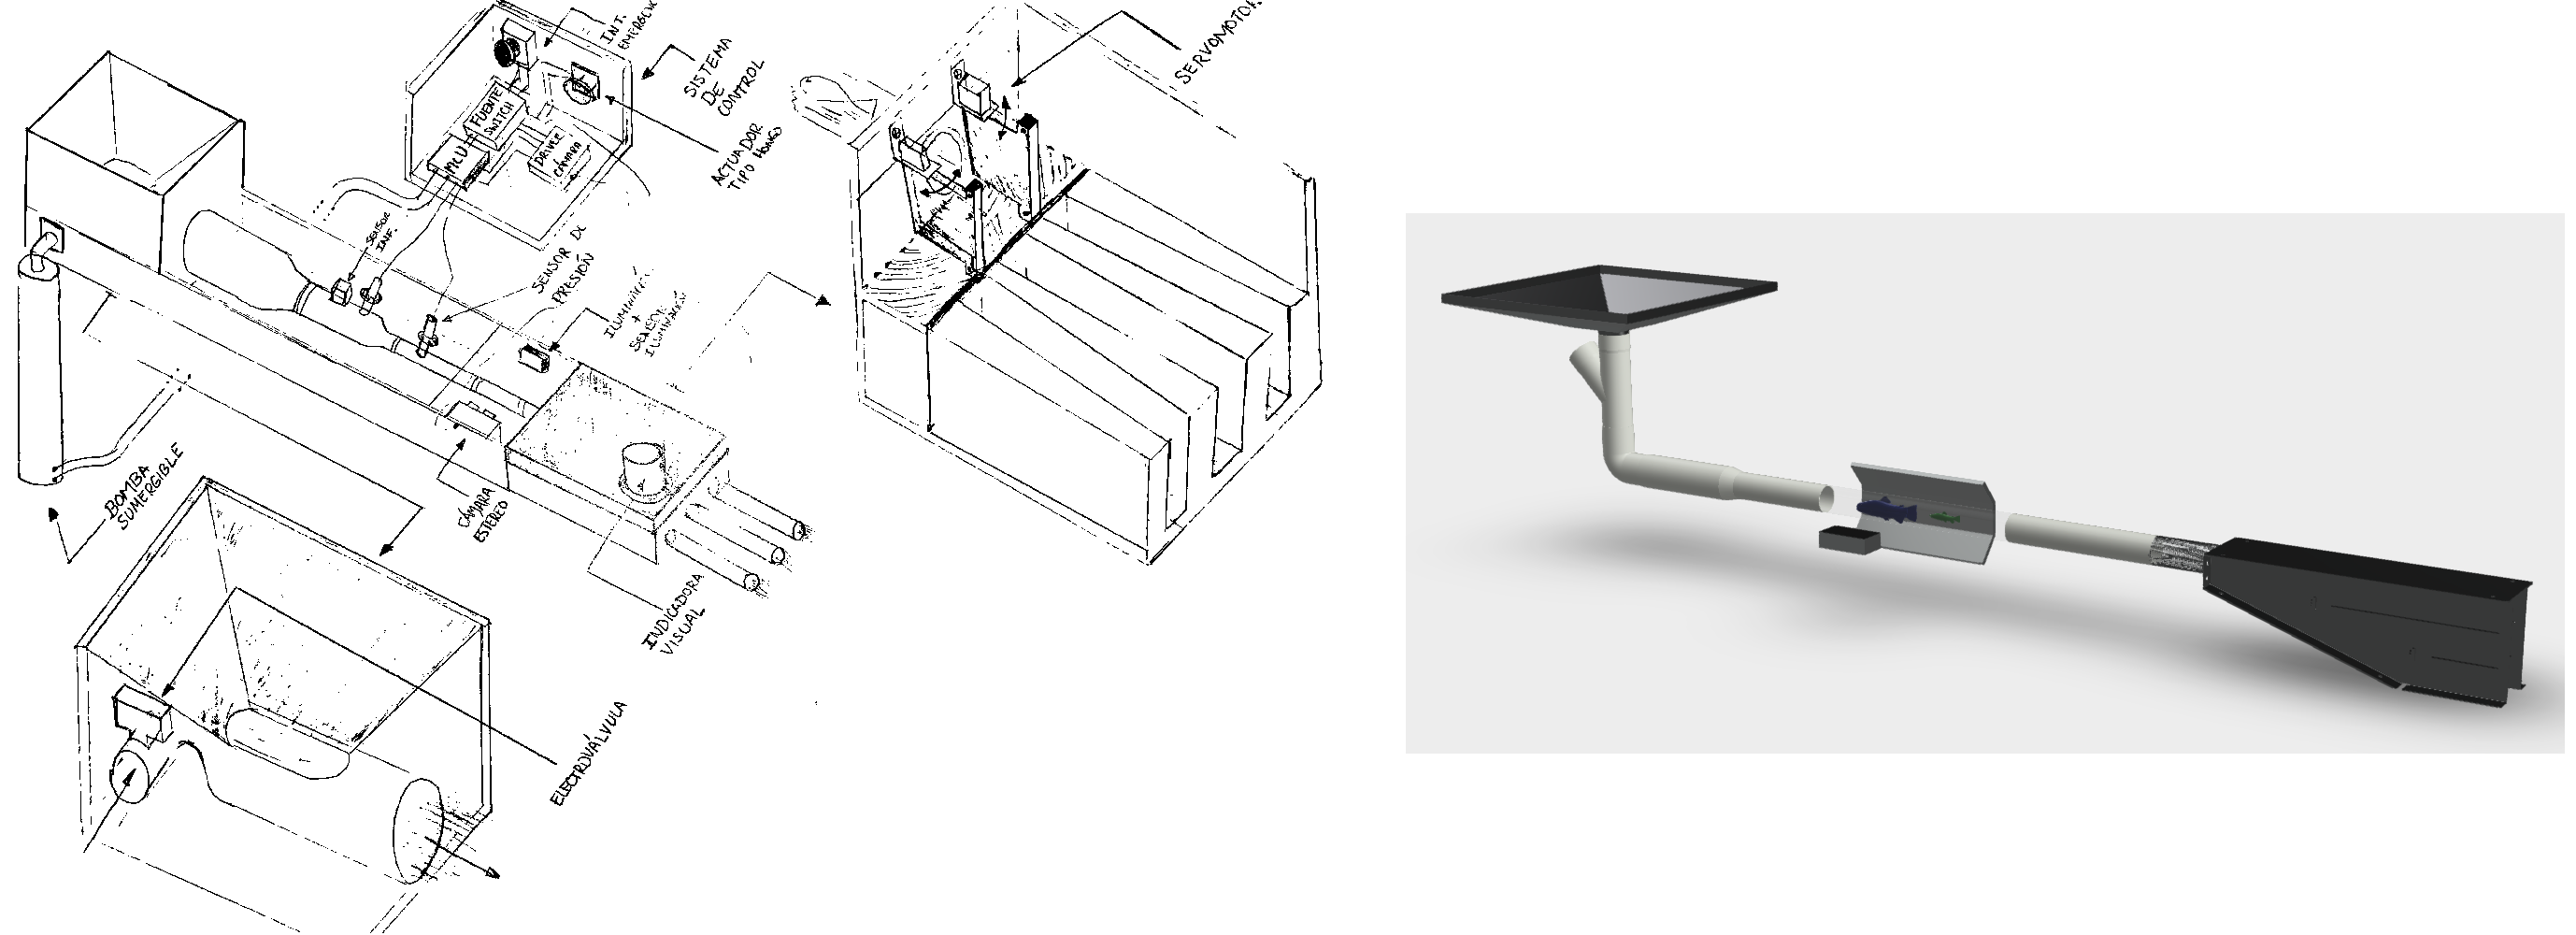
\includegraphics[width=1\textwidth]{chapter4/concepto optimo dibujo y virtual.png}
	\caption{Dibujo del concepto óptimo}
	\begin{myflushleftportland}
		Fuente: \cite{DiazVergara2020}.
	\end{myflushleftportland}
	\label{fig:concepto optimo dibujo y virtual}
\end{myfigure}

El desarrollo de ingeniería del concepto se realizó en el programa \textit{Fusion 360}\footnote{"Integrated CAD, CAM, CAE, and PCB software". Enlace:https://www.autodesk.com/products/fusion-360/overview}. Tanto los diseños como renders\footnote{Imágenes procesadas de un diseño para ser foto-realistas.} pueden ser visualizados en su última versión de manera online gracias al software. En el presente trabajo se brindarán dichos enlaces a modo de pie de página.

%% NUEVO SUBSECCION X.X
\section{Objetivos}

Se presenta el objetivo general y los objetivos específicos del presente trabajo.

%% NUEVA SUB-SUB-SECCION X.X.X
\subsection{Objetivo general}

Realizar el diseño integral de un sistema clasificador y contador de truchas arcoíris de 15 a 20 centímetros a partir del diseño conceptual previo.

%% NUEVA SUB-SUB-SECCION X.X.X
\subsection{Objetivos específicos}

\begin{itemize}
	\item Recolectar imágenes para formar una base de datos de truchas.
	\item Desarrollar el procesamiento de imágenes para la detección y conteo de truchas arcoíris.
	\item Orientar el desarrollo del proyecto hacia una máquina de bajo costo y con durabilidad.
	\item Simular 	
	
\end{itemize}


%% NUEVA SECCIÓN X.X
\section{Alcance}

Dolor sit amet consectetur adipiscing elit ut aliquam purus sit. Dolor sed viverra ipsum nunc aliquet bibendum. Euismod in pellentesque massa placerat. Et malesuada fames ac turpis egestas sed tempus urna. Euismod elementum nisi quis eleifend quam adipiscing vitae proin. Ornare suspendisse sed nisi lacus sed. Mollis aliquam ut porttitor leo a diam.

